\subsection{Firewall Script}
\begin{figure}[htp]
\centering
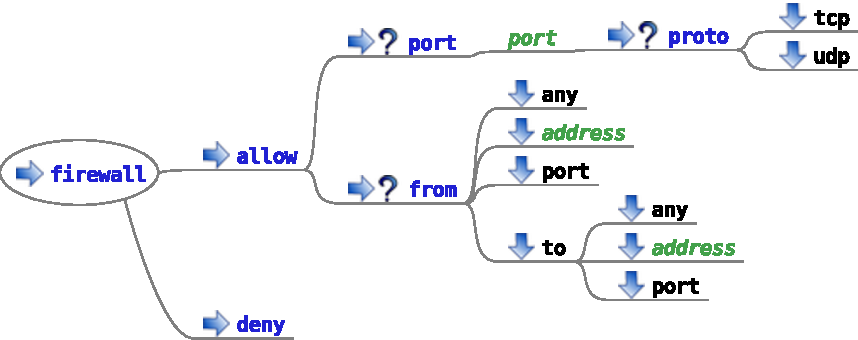
\includegraphics[width=0.7\textwidth]{firewall_service_script}
\label{fig:firewall_script_statements}
\caption{Firewall Script Statements}
\end{figure}


%% firewall
\TheStatement{firewall}
\TheStatement*[firewall]{firewall \{ allow deny \}}

Entry point in the firewall script.

%% allow
\TheStatement[firewall:allow]{allow}
\TheStatement*[firewall!allow]{allow [[port] [, proto]] [from [, port] [, proto]]}

Allow packets from the source host, port and protocol to the destination
host, port and protocol. Without any arguments sets the default mode for the 
firewall to allow all.

%% deny
\TheStatement[firewall:deny]{deny}
\TheStatement*[firewall!deny]{deny [[port] [, proto]] [from [, port] [, proto]]}

Denies packets from the source host, port and protocol to the destination
host, port and protocol.
Without any arguments sets the default mode for the firewall to deny all.

%% port
\TheStatement[firewall:port]{port}
\TheStatement*[firewall!port]{port \Arg{port}}

Sets the \Arg{port} number or service name to allow or deny packets from.

%% proto
\TheStatement[firewall:proto]{proto}
\TheStatement*[firewall!proto]{proto tcp|udp}

Sets the Internet protocol to allow or deny packets from. If no protocol
is set TCP and UDP is assumed.

\begin{compactdesc}
\item[tcp] TCP/IP protocol.
\item[udp] UDP/IP protocol.
\end{compactdesc}

%% from
\TheStatement[firewall:from]{from}
\TheStatement*[firewall!from]{from any|\Arg{address}}

Sets the host as the source. Keyword \qcode{any} means from any host.

%% to
\TheStatement[firewall:to]{to}
\TheStatement*[firewall!to]{to any|\Arg{address} [, port] [, proto]}

Sets the host as the destination. Keyword \qcode{any} means from any host.

